% ══════════════════════════════════════════════════════════════════════════════
% 期末報告（中文）— 封面與目錄，內容章節待自期中報告移植
% 編譯方式：LuaLaTeX，見 .latexmkrc
% ══════════════════════════════════════════════════════════════════════════════
\documentclass[12pt,fontset=none]{ctexart}

% ── Packages ──────────────────────────────────────────────────────────────────
\usepackage[margin=1in]{geometry}
\usepackage{amsmath, amssymb}
\usepackage{graphicx}
\usepackage{booktabs}
\usepackage[hidelinks]{hyperref}
\usepackage{caption}

% ── CJK font: DFKai-SB (標楷體) on Windows, falling back to AR PL KaitiM Big5
% (a metric/style-compatible open Kaiti substitute) when DFKai-SB isn't
% installed (e.g. Linux: apt install fonts-arphic-bkai00mp).
% fontset=none disables ctex's auto-detected Simplified-Chinese fonts
% (SimHei/KaiTi), which aren't installed on this Traditional-Chinese system.
\IfFontExistsTF{DFKai-SB}{%
  \setCJKmainfont{DFKai-SB}
  \setCJKsansfont{DFKai-SB}
  \setCJKmonofont{DFKai-SB}
}{%
  \setCJKmainfont{AR PL KaitiM Big5}
  \setCJKsansfont{AR PL KaitiM Big5}
  \setCJKmonofont{AR PL KaitiM Big5}
}

% ── Traditional-Chinese wording overrides ──────────────────────────────────────
% ctex's built-in auto-generated names (contentsname/figurename/refname)
% default to Simplified Chinese; override them for a Traditional document.
\renewcommand{\contentsname}{目錄}
\renewcommand{\figurename}{圖}
\renewcommand{\refname}{參考文獻}

% ── Metadata ──────────────────────────────────────────────────────────────────
\title{星載合成孔徑雷達船舶偵測之建模與評估\\期末報告}
\author{陳仁澤}
\date{\today}

% plain: no running header (section name), just the page number, centered
% at the bottom -- overrides ctexart's default "headings" style.
\pagestyle{plain}

\begin{document}

% ── Cover page ──────────────────────────────────────────────────────────────
% Custom titlepage (instead of \maketitle) to show the funded project name,
% PI, research assistant, and execution period alongside the report title.
\begin{titlepage}
  \centering
  \vspace*{2cm}
  {\LARGE\bfseries 計畫名稱：基於壓縮感測之合成孔徑雷達即時成像演算法\par}
  \vspace{1.5cm}
  {\Large 星載合成孔徑雷達船舶偵測之建模與評估\par}
  {\Large 期末報告\par}
  \vspace{4cm}
  {\large
    \begin{tabular}{r@{\hspace{0.5em}}l}
      計畫主持人： & 國立台灣大學重點科技學院\ 蔡佩芸 \\[0.6em]
      研究助理：   & 陳仁澤 \\[0.6em]
      執行期間：   & 2026/3 -- 2027/2 \\
    \end{tabular}
  }
  \vfill
\end{titlepage}

\tableofcontents

\newpage
% ══════════════════════════════════════════════════════════════════════════════
\section{緒論與研究動機}

\subsection{背景}
合成孔徑雷達（SAR）原始資料透過下傳鏈路傳送至地面站，並在地面完成聚焦成像、影像強化與船舶偵測；偵測到的船舶目標可提供海事監控所需的位置與目標資訊。

\begin{figure}[htbp]
  \centering
  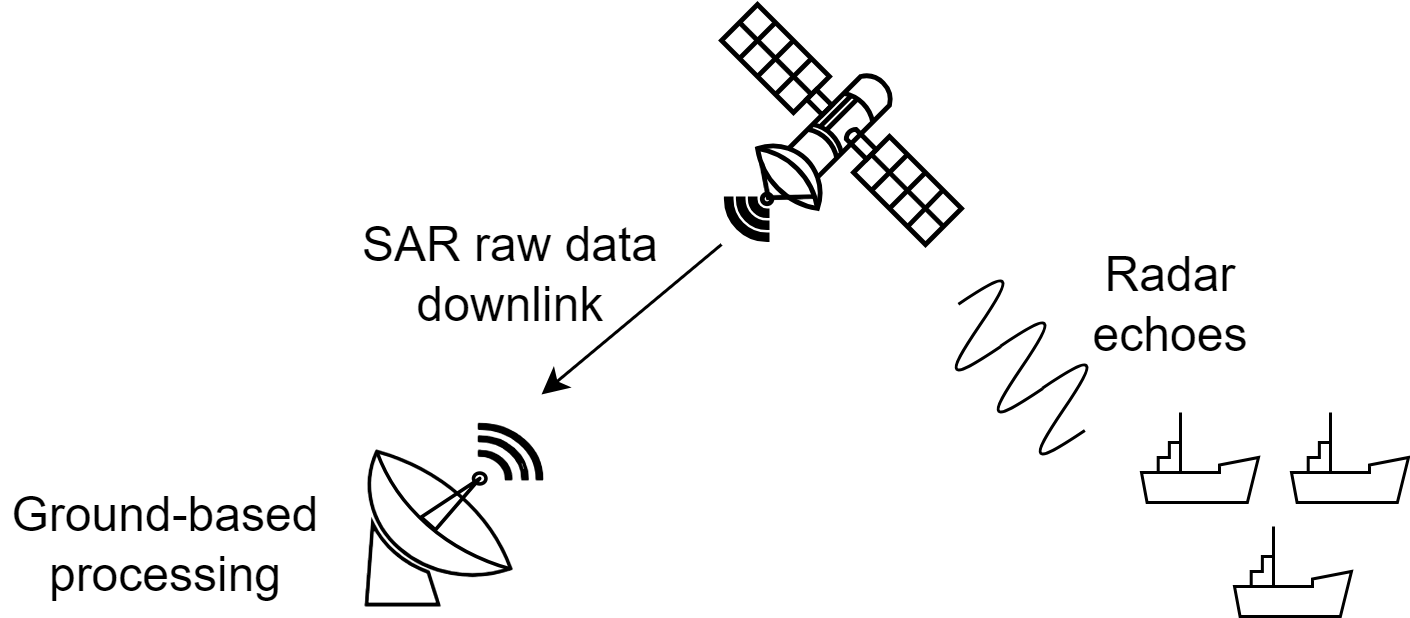
\includegraphics[width=0.6\textwidth]{../../04_group_meeting/figures/intro/ground_based_sar_ship_detection.png}
  \caption{地面式 SAR 船舶偵測處理流程示意圖。}
\end{figure}

本計畫的核心精神，是利用壓縮感測（Compressed Sensing, CS）理論：若待重建訊號具有稀疏性（sparsity），便可透過稀疏正則化準確重建 \cite{donoho_cs, candes_cs}：
\begin{equation}
  \hat{\mathbf{H}} = \arg\min_{\mathbf{H}}
    \underbrace{\frac{1}{2}\left\|\mathbf{Y} - \mathcal{A}(\mathbf{H})\right\|_F^2}_{\text{符合觀測到的回波}}
    + \lambda \underbrace{R(\mathbf{H})}_{\text{稀疏性限制}}
  \label{eq:cs-formulation}
\end{equation}
其中 $\mathbf{Y}$ 為原始回波、$\mathbf{H}$ 為待重建之場景反射率影像、$\mathcal{A}(\cdot)$ 為成像前向算子（見 4.2 節），$R(\mathbf{H})$ 為稀疏誘導正則項。

海面 SAR 場景恰好符合此稀疏性假設：海面雜訊背景均勻、反射率低，船舶則是少數強散射點，使場景反射率 $\mathbf{H}$ 本身即具稀疏結構。這也是本研究以「船舶偵測」作為評估任務的原因：偵測表現的提升與否，可直接反映稀疏正則化（式 \eqref{eq:cs-formulation}）強化 SAR 影像的實際效益。

\subsection{問題與動機}
本研究欲解決以下問題：
\begin{itemize}
  \item 地面式處理：原始資料量大、下傳頻寬有限，導致目標資訊延遲。
  \item 星載（onboard）處理：僅需下傳偵測到的目標資訊而非完整原始資料，可降低下傳鏈路頻寬需求，並縮短從下傳到地端處理完成的延遲，但受限於運算能力、記憶體與功耗。
  \item Speckle noise 干擾：SAR 屬同調成像系統，影像中不可避免存在乘性 speckle noise；雜訊亮點可能被誤判為船舶（false positive），也可能掩蓋真實的弱散射目標（false negative），須加以抑制才能確保偵測結果可信。
\end{itemize}
上述問題中，星載運算資源有限與 speckle noise 抑制看似為兩個獨立需求，但壓縮感測可一併回應：真實場景反射率本身是稀疏的（見 1.1 節），而 speckle noise 是疊加在每個像素上的乘性擾動，會使原本接近零的背景像素被抬高、變得雜訊化；式 \eqref{eq:cs-formulation} 之稀疏正則化利用場景稀疏的先驗，將振幅低（多為雜訊擾動的背景）的像素壓制為零，同時保留振幅本來就高的目標像素，因此能以同一套輕量化框架兼顧抑制 speckle noise 與低運算量兩項需求。

\subsection{研究目標}
本計畫原訂之研究範疇涵蓋 speckle 統計建模與噪聲注入模擬、以壓縮感測為基礎的即時 SAR 成像、去斑（despeckle）方法比較、以及以 YOLO 為基礎之船舶偵測評估等階段。本節之研究目標即回應 1.2 節所列之三項痛點：

\begin{itemize}
  \item 即時性之必要性：船舶偵測若僅能於地面事後處理完成，則難以支援即時海事監控需求；成像方法須兼顧運算效率，使其可行於星載平台之算力與功耗限制下，方能達成低延遲之目標資訊回傳。
  \item 為何引入壓縮感測：如 1.1、1.2 節所述，星載平台受限於運算資源，須採用輕量化的成像方法；而壓縮感測之稀疏正則化機制，天然具備抑制 speckle noise 的能力。因此壓縮感測可同時回應「低運算量」與「speckle noise 抑制」兩項需求，是本計畫選擇以其為核心方法的原因。
  \item 如何處理 speckle noise：規劃先以統計方式建模 SAR 影像中 speckle noise 的分布與 number of looks 等參數，並將其注入模擬回波中，以在具真實統計特性的資料上，比較稀疏正則化與傳統去斑方法之效果。
\end{itemize}

\newpage
上述痛點與研究目標之關係，以及各階段工作項目如何串接，如圖 \ref{fig:research-goal-diagram} 所示。

\begin{figure}[htbp]
  \centering
  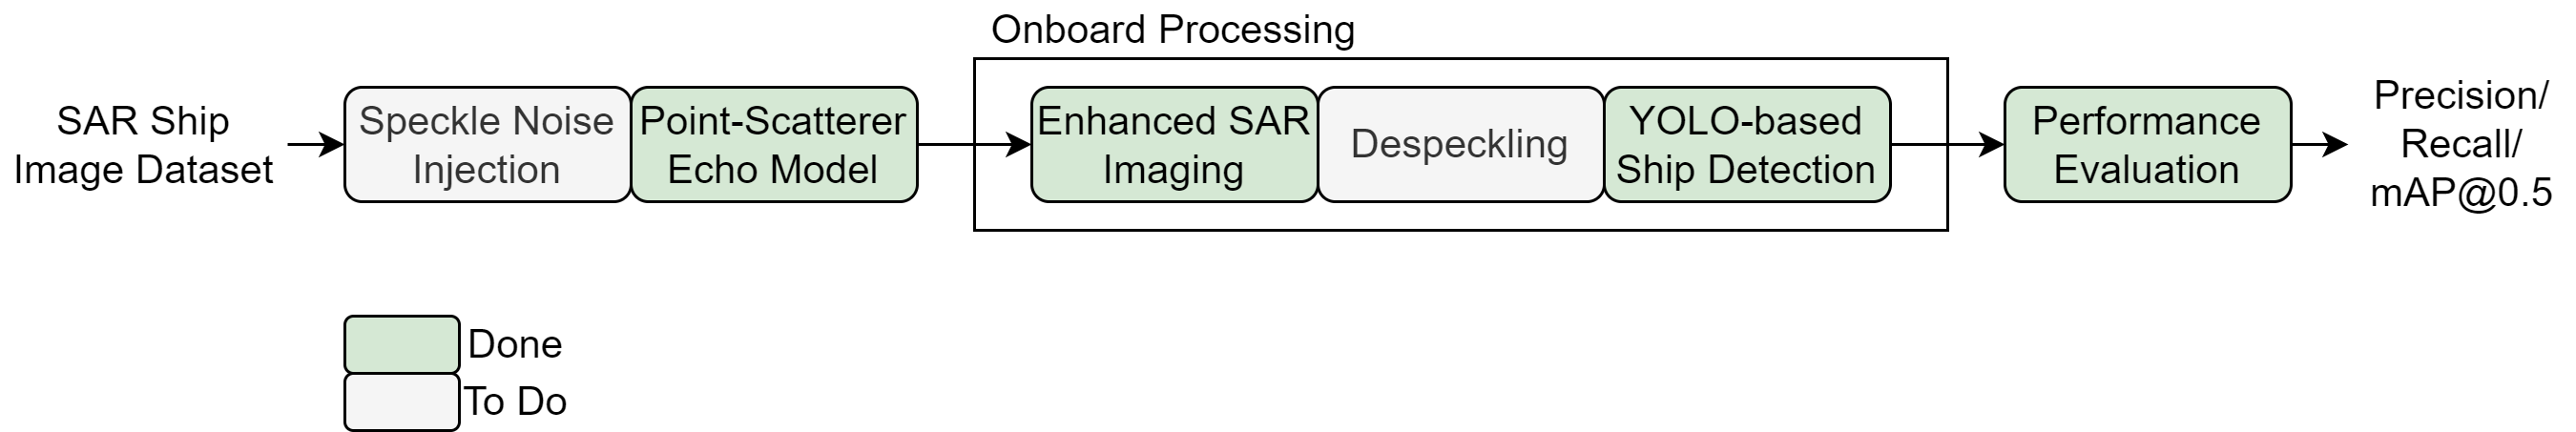
\includegraphics[width=\textwidth]{../../04_group_meeting/figures/intro/flow.png}
  \caption{研究目標概念圖：由 SAR 船舶影像資料集出發，經 speckle noise 注入與點散射體回波模型模擬，送入星載（onboard）處理流程——強化 SAR 成像、去斑、YOLO 船舶偵測——最終產出 Precision/Recall/mAP@0.5 等效能指標（指標定義詳見 3.3 節）。圖中綠色標示已完成之工作項目，灰色標示尚未完成之項目。}
  \label{fig:research-goal-diagram}
\end{figure}

% ══════════════════════════════════════════════════════════════════════════════
\section{文獻探討}

\subsection{壓縮感測於 SAR 影像重建之應用}
稀疏正則化已廣泛用於 SAR 影像重建，但訴求多為提升重建影像品質，而非下游應用任務：
\begin{itemize}
  \item Bi \textit{et al.} \cite{sparse_sar_imaging}：$\ell_1$ 正則化＋soft-thresholding，訴求降低運算複雜度以利即時成像。
  \item Zhang \textit{et al.} \cite{zhang_reweighted}：multi-segment-reweighted 正則化，訴求改善 $\ell_1$ 造成的振幅失真。
  \item Liu \textit{et al.} \cite{liu_compound_reg}：$\ell_{1/2}$＋TV 複合正則化，訴求處理低過採樣資料並保留空間結構。
\end{itemize}
三者皆以影像品質指標評估，未涉及下游偵測任務。

\subsection{SAR 船舶偵測之既有研究}
近期研究多將 speckle noise 抑制放在偵測網路的特徵層級，而非影像域：
\begin{itemize}
  \item SARES-DEIM \cite{sares_deim}：DETR + Mixture-of-Experts，特徵層級抑制 speckle noise，於 HRSID 上 mAP@0.5:0.95 由 YOLOv11 之 67.7\% 提升至 76.4\%。
  \item CVMT \cite{cvmt}：雙分支複數值 Transformer，以 Super Feature Learning 於特徵層級抑制雜訊，於 OpenSARShip / FAIR-CSAR 達 SOTA。
\end{itemize}
兩者皆以已成像影像為輸入、採大型 Transformer 架構，訓練與推論成本高。

\subsection{本研究之定位與差異性}
本研究將稀疏正則化直接嵌入「回波 $\to$ 成像 $\to$ 稀疏精修」流程，並以船舶偵測表現（Precision/Recall/mAP@0.5）評估其效益——相較 2.1 節僅評估影像品質，本研究更貼近實際應用；相較 2.2 節之 Transformer 架構，本研究改用計算量低廉、具封閉解的 $\ell_1$ soft-thresholding 搭配輕量化 YOLO，較適合星載平台之算力限制。

可能缺點：目前僅用影像域 $\ell_1$ 正則化，尚未與特徵層級抑制或傳統去斑濾波器比較，其在近岸雜訊、小型目標上的效果仍待驗證。

% ══════════════════════════════════════════════════════════════════════════════
\section{評估架構}

\subsection{整體評估流程}
本研究聚焦於「強化 SAR 成像」，並以 YOLO-based 船舶偵測作為評估任務，整體流程如圖 \ref{fig:eval-framework} 所示：從點散射體回波模型產生原始回波，經過強化 SAR 成像後，再送入 YOLO 偵測模型評估表現。

\begin{figure}[htbp]
  \centering
  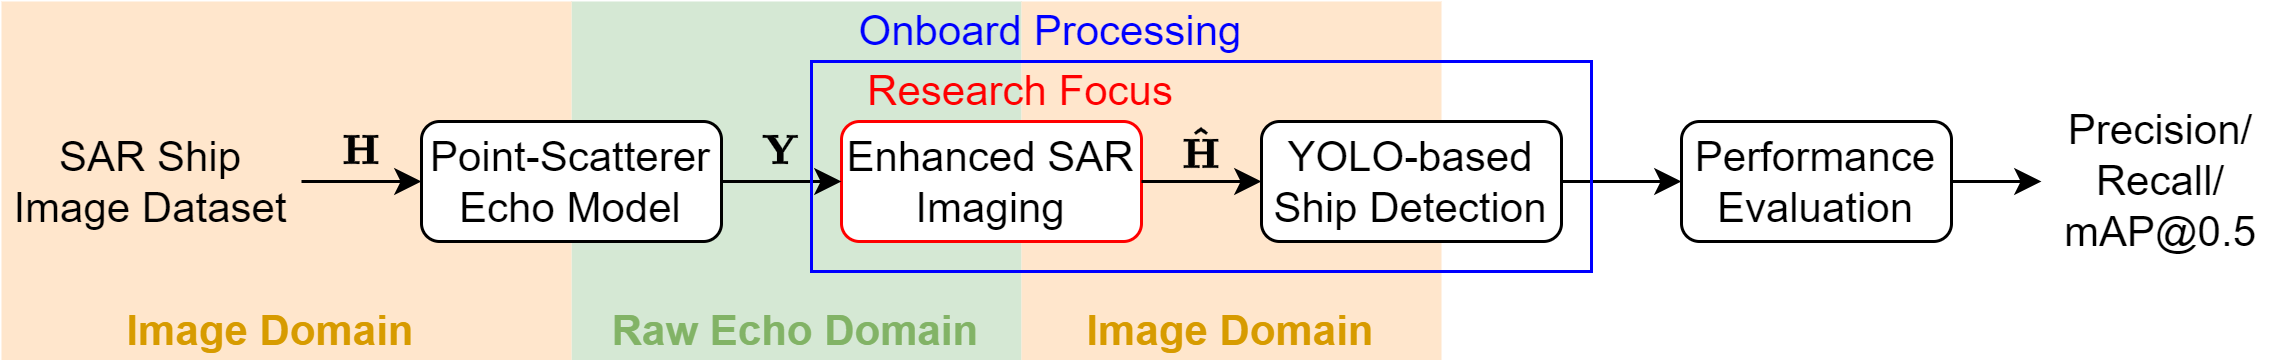
\includegraphics[width=\textwidth]{../../04_group_meeting/figures/pipeline/evaluation_framework.png}
  \caption{評估架構管線}
  \label{fig:eval-framework}
\end{figure}

\subsection{資料集與偵測模型設定}
本研究使用 HRSID（High-Resolution SAR Images Dataset）資料集 \cite{hrsid}：
\begin{itemize}
  \item 訓練集：3,642 張影像；驗證集：1,962 張影像
  \item 影像尺寸：$800 \times 800$ 像素
\end{itemize}
偵測模型採用 YOLO11m，於 HRSID 上微調訓練 100 個 epoch，驗證表現如表 \ref{tab:val-perf}。

\begin{table}[htbp]
  \centering
  \caption{YOLO11m 於 HRSID 驗證集上的表現。}
  \label{tab:val-perf}
  \begin{tabular}{lc}
    \toprule
    指標 & 數值 \\
    \midrule
    Precision & 0.910 \\
    Recall    & 0.840 \\
    mAP@0.5   & 0.922 \\
    \bottomrule
  \end{tabular}
\end{table}

\begin{figure}[htbp]
  \centering
  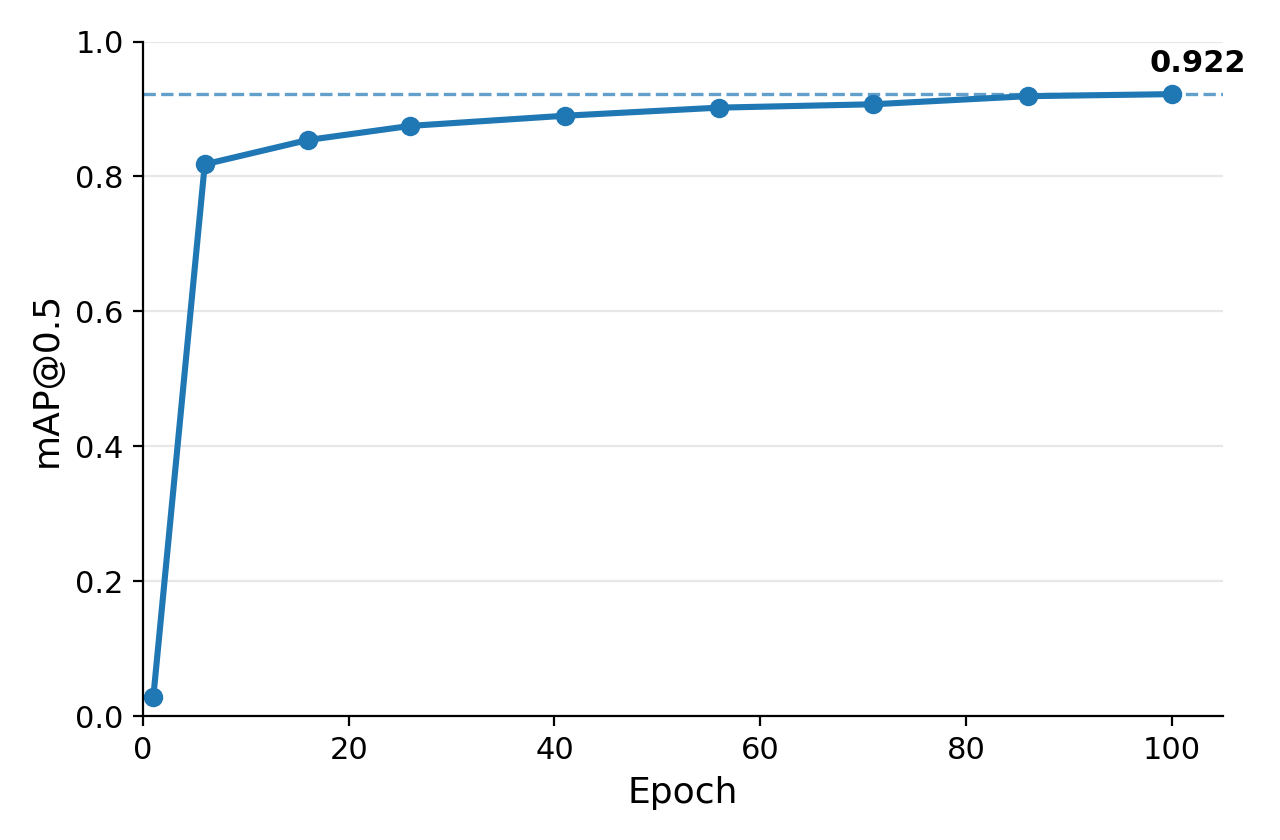
\includegraphics[width=0.6\textwidth]{../../04_group_meeting/figures/yolo/map_vs_epoch.png}
  \caption{訓練過程中 mAP@0.5 隨 epoch 數的變化。}
\end{figure}

\subsection{評估指標}
\begin{itemize}
  \item Precision $= \dfrac{TP}{TP+FP}$，Recall $= \dfrac{TP}{TP+FN}$
  \begin{itemize}
    \item[] TP：True Positive；FP：False Positive；FN：False Negative
  \end{itemize}
  \item mAP@0.5：在 IoU 門檻值 0.5 下，跨類別的平均精確度（Mean Average Precision）
  \begin{itemize}
    \item[] IoU（Intersection over Union）＝ 預測框與真實框的重疊面積 / 聯集面積
  \end{itemize}
\end{itemize}

\begin{figure}[htbp]
  \centering
  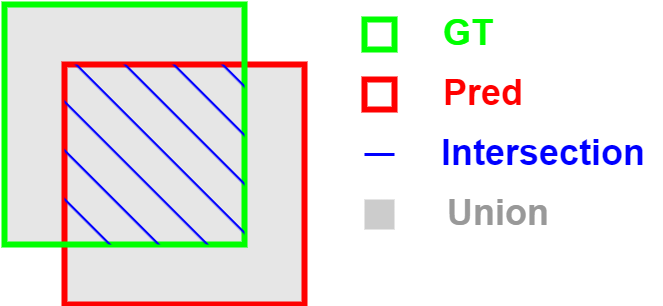
\includegraphics[width=0.35\textwidth]{../../04_group_meeting/figures/pipeline/iou_def.png}
  \caption{IoU 定義示意圖：GT 為真實標註框，Pred 為預測框，IoU＝交集（Intersection）面積除以聯集（Union）面積。}
\end{figure}
上述指標定義參考自文獻 \cite{sares_deim}。

\subsection{YOLO 船舶偵測結果}
在 HRSID 驗證集（1,962 張影像，其中近岸 369 張、離岸 1,593 張）上，依場景分類的偵測結果如表 \ref{tab:yolo-results} 所示；離岸場景的偵測表現優於近岸場景 \cite{balance_scene}。
表 \ref{tab:val-perf} 使用 GPU 進行 inference，表 \ref{tab:yolo-results} 改用 CPU 進行 inference，因此兩表數值略有差異；表 \ref{tab:yolo-results} 之後的所有實驗皆使用 CPU 進行 inference。近岸與離岸場景之偵測範例如圖 \ref{fig:gt-vs-pred} 所示。

\begin{table}[htbp]
  \centering
  \caption{YOLO 船舶偵測結果（依場景分類）。}
  \label{tab:yolo-results}
  \begin{tabular}{lccc}
    \toprule
     & 全體 & 近岸 & 離岸 \\
    \midrule
    影像數    & 1,962 & 369   & 1,593 \\
    Precision & 0.913 & 0.803 & 0.982 \\
    Recall    & 0.846 & 0.741 & 0.965 \\
    mAP@0.5   & 0.918 & 0.817 & 0.984 \\
    \bottomrule
  \end{tabular}
\end{table}

\begin{figure}[htbp]
  \centering
  \begin{minipage}{0.48\textwidth}
    \centering
    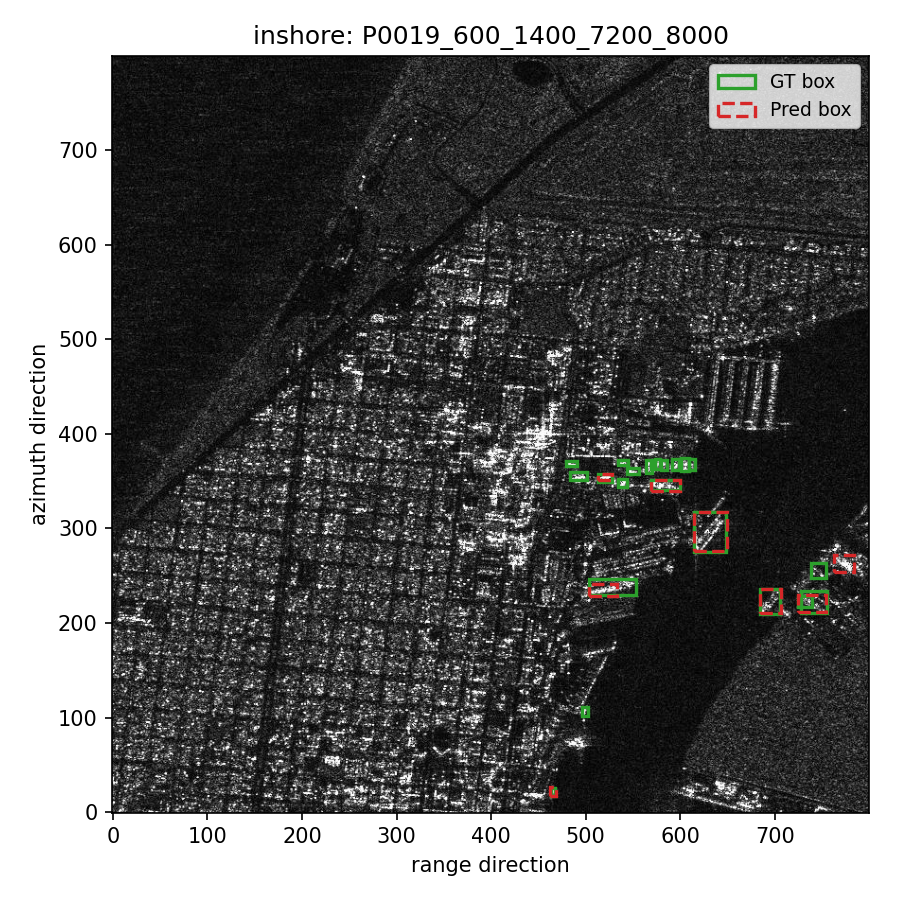
\includegraphics[width=\linewidth]{../../04_group_meeting/figures/yolo/inshore_example_gt_vs_pred.png}
    \caption*{近岸範例}
  \end{minipage}
  \hfill
  \begin{minipage}{0.48\textwidth}
    \centering
    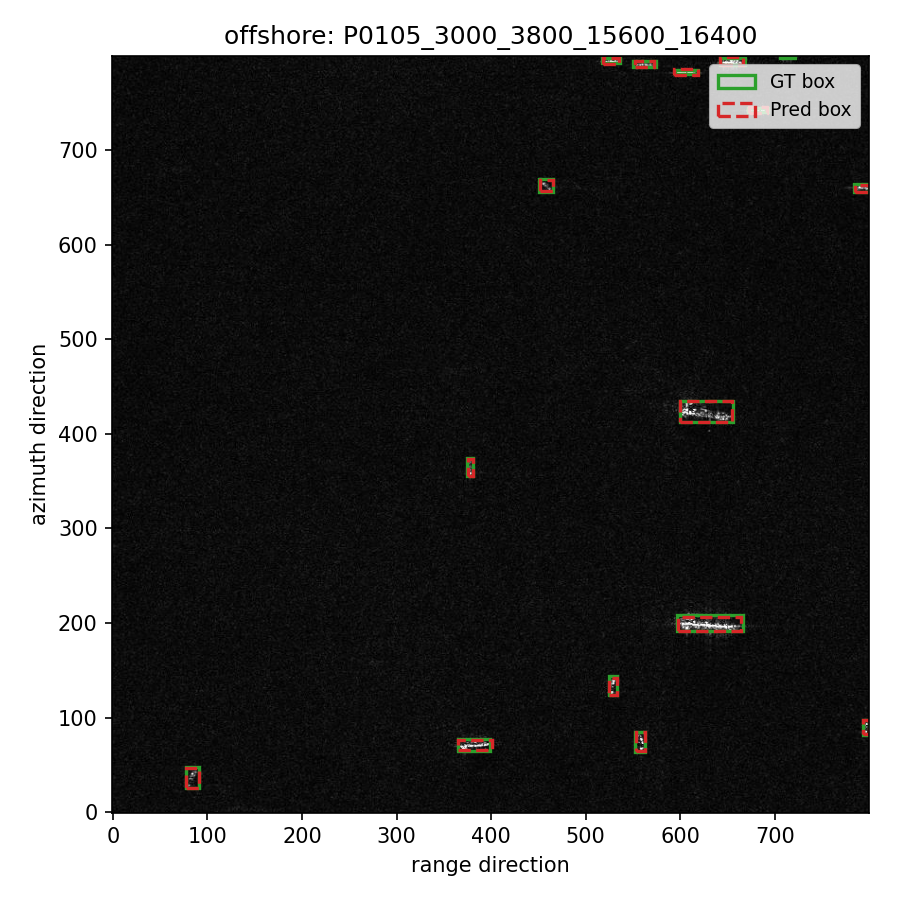
\includegraphics[width=\linewidth]{../../04_group_meeting/figures/yolo/offshore_example_gt_vs_pred.png}
    \caption*{離岸範例}
  \end{minipage}
  \caption{真實標註框（GT）與預測框（Pred）比較範例。}
  \label{fig:gt-vs-pred}
\end{figure}

\newpage
% ══════════════════════════════════════════════════════════════════════════════
\section{SAR 回波與成像模型}

\subsection{點散射體回波模型：幾何關係}
\label{subsec:point-scatterer}
輸入 SAR 影像中每個像素的 range location（行）、azimuth location（列）與 intensity（強度值），分別轉換為對應散射體的 range、Doppler（即下述之距離偏移 $d_k$、方位時間偏移 $\Delta\eta_k$）與 magnitude（散射係數 $A_k$，見下節訊號合成）。成像於斜距（slant range）方向進行，像素對應的距離偏移即為散射體 $k$ 之斜距偏移 $d_k$。

目標位置決定了隨慢時間 $\eta_m$ 變化的斜距 $R_k(\eta_m)$：
\begin{equation}
  R_k(\eta_m) = \sqrt{R_{0,k}^2 + (\eta_m + \Delta\eta_k)^2 V_r^2}
\end{equation}
其中 $R_{0,k} = R_0 + d_k$：
\begin{itemize}
  \item $R_0$：場景中心的斜距
  \item $d_k$：散射體 $k$ 相對場景中心之斜距方向距離偏移
  \item $\eta_m = m\Delta\eta$：慢時間
  \item $\Delta\eta_k$：散射體 $k$ 相對場景中心的方位時間偏移
\end{itemize}

\begin{figure}[htbp]
  \centering
  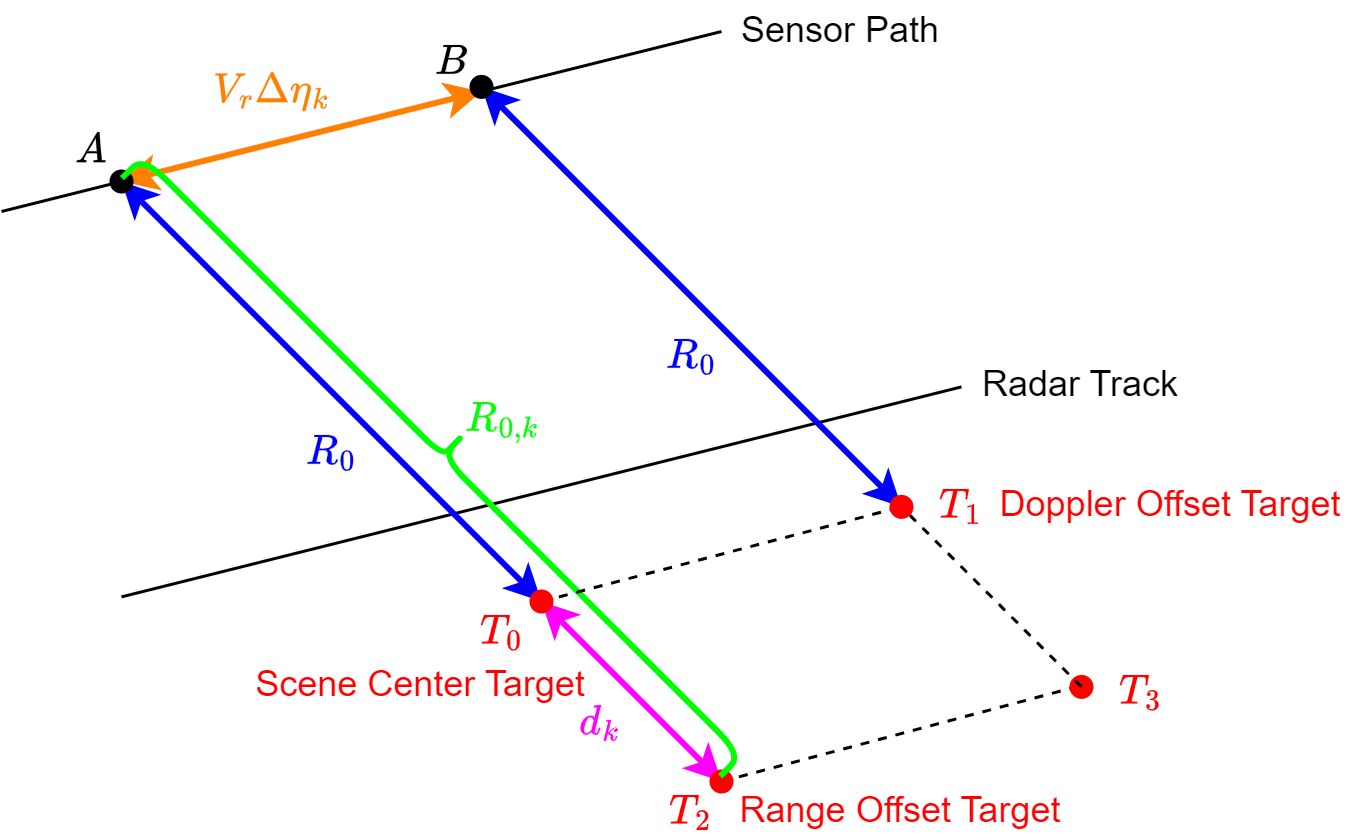
\includegraphics[width=0.55\textwidth]{../../04_group_meeting/figures/point_scatterer/point_target_geometry.png}
  \caption{點散射體回波模型幾何關係示意圖。}
\end{figure}

\subsection{訊號合成}
延遲與相位皆為幾何相依：
\begin{equation}
  \tau_k(\eta_m) = \frac{2R_k(\eta_m)}{c}, \qquad
  \phi_k(\eta_m) = -4\pi \frac{R_k(\eta_m)}{\lambda}
\end{equation}
回波訊號矩陣 $\mathbf{S} = [s_{m,n}]_{M\times N}$ 由下式合成：
\begin{equation}
  s_{m,n} = \sum_k A_k\,\mathrm{rect}\!\left(\frac{\tau_n - \tau_k(\eta_m)}{T_r}\right)
    \cdot e^{j\pi K_r\left(\tau_n - \tau_k(\eta_m)\right)^2}
    \cdot e^{j\phi_k(\eta_m)}
\end{equation}
其中：
\begin{itemize}
  \item $\eta_m = m\Delta\eta$：慢時間；$\tau_n = n\Delta\tau$：快時間
  \item $A_k$：散射體 $k$ 的散射係數
  \item $K_r = B_r / T_r$：chirp 調頻率；$B_r$：chirp 頻寬（Hz）；$T_r$：脈衝時寬（秒）
\end{itemize}
$\mathbf{S}$ 與場景反射率 $\mathbf{H}$ 皆為複數值 $M \times N$ matrix。接收到的回波為 $\mathbf{Y} = \mathbf{S} + \mathbf{W}$，其中 $\mathbf{W}$ 為熱噪聲（thermal noise），模型化為 i.i.d.\ circular complex Gaussian；目前實驗中 $\mathbf{W}$ 設為零，即 $\mathbf{Y} = \mathbf{S}$。

% ══════════════════════════════════════════════════════════════════════════════
% 以下章節內容待自 document/05_industry_academia_collaboration/midterm/report.tex 移植。

% ══════════════════════════════════════════════════════════════════════════════
\begin{thebibliography}{9}

\bibitem{donoho_cs}
D. L. Donoho, ``Compressed Sensing,'' in \textit{IEEE Transactions on Information Theory}, vol. 52, no. 4, pp. 1289--1306, April 2006.

\bibitem{candes_cs}
E. J. Cand\`es, J. Romberg and T. Tao, ``Robust Uncertainty Principles: Exact Signal Reconstruction from Highly Incomplete Frequency Information,'' in \textit{IEEE Transactions on Information Theory}, vol. 52, no. 2, pp. 489--509, February 2006.

\bibitem{sares_deim}
F. Song, S. Yang and X. Zhou, ``SARES-DEIM: Sparse Mixture-of-Experts Meets DETR for Robust SAR Ship Detection,'' in \textit{IEEE Journal of Selected Topics in Applied Earth Observations and Remote Sensing (JSTARS)}, 2026.

\bibitem{hrsid}
S. Wei, X. Zeng, Q. Qu, M. Wang, H. Su and J. Shi, ``HRSID: A High-Resolution SAR Images Dataset for Ship Detection and Instance Segmentation,'' in \textit{IEEE Access}, vol. 8, pp. 120234--120254, 2020.

\bibitem{balance_scene}
T. Zhang \textit{et al.}, ``Balance Scene Learning Mechanism for Offshore and Inshore Ship Detection in SAR Images,'' in \textit{IEEE Geoscience and Remote Sensing Letters}, vol. 19, pp. 1--5, 2022.

\bibitem{sparse_sar_imaging}
H. Bi, G. Bi, B. Zhang, W. Hong and Y. Wu, ``From Theory to Application: Real-Time Sparse SAR Imaging,'' in \textit{IEEE Transactions on Geoscience and Remote Sensing}, vol. 58, no. 4, pp. 2928--2936, April 2020.

\bibitem{zhang_reweighted}
Y. Zhang, B. Zhang and Y. Wu, ``Undistorted and Consistent Enhancement of Automotive SAR Image via Multi-Segment-Reweighted Regularization,'' in \textit{Remote Sensing}, vol. 17, no. 9, Art. no. 1483, April 2025.

\bibitem{liu_compound_reg}
M. Liu, J. Pan, J. Zhu, Z. Chen, B. Zhang and Y. Wu, ``A Sparse SAR Imaging Method for Low-Oversampled Staggered Mode via Compound Regularization,'' in \textit{Remote Sensing}, vol. 16, no. 8, Art. no. 1459, April 2024.

\bibitem{cvmt}
K. Ni, P. Wang, Z. Zheng and Y. Zhong, ``Complex-Value Transformer for SAR Ship Detection,'' in \textit{ISPRS Journal of Photogrammetry and Remote Sensing}, 2026.

\bibitem{cumming_wong}
I. G. Cumming and F. H. Wong, \textit{Digital Processing of Synthetic Aperture Radar Data: Algorithms and Implementation}, Artech House, 2005.

\end{thebibliography}

\end{document}
